\documentclass[
  %fleqn,     das ist für die zentrierung
	parskip=half,
	captions=tableheading,
  titlepage=firstiscover, 		%************************************************** by Rk
	bibliography=totoc		%*************************************by Rk
	]{scrartcl}			
% \usepackage{etex}
% \reserveinserts{28}

%Das ist für die Kopfzeile
\usepackage[headsepline]{scrlayer-scrpage}
\pagestyle{scrheadings}
\clearpairofpagestyles
\ofoot{\pagemark}
\ohead{\headmark}
\automark{section}

% Warnung, falls nochmal kompiliert werden muss		%*************************************by Rk
\usepackage[aux]{rerunfilecheck}

% unverzichtbare Mathe-Befehle
\usepackage{amsmath}
% viele Mathe-Symbole
\usepackage{amssymb}
% Erweiterungen für amsmath
\usepackage{mathtools}
\usepackage{upgreek}
% Fonteinstellungen
\usepackage{fontspec}				%************************************************** by Rk
% Latin Modern Fonts werden automatisch geladen
% Latin Modern Fonts werden automatisch geladen
% Alternativ zum Beispiel:
%\setromanfont{Libertinus Serif}
%\setsansfont{Libertinus Sans}
%\setmonofont{Libertinus Mono}

\usepackage{polyglossia}
\usepackage[				%************************************************** by Rk
	backend=biber,
]{biblatex}  	
%Quellendatenbank	
\setmainlanguage{german}			
\addbibresource{lit.bib}		%************************************************** by Rk


\usepackage{expl3}
\usepackage{xparse}

\usepackage{physics}

\usepackage[unicode, german]{hyperref}
\usepackage[autostyle]{csquotes}
\usepackage[
  math-style=ISO,    % ┐
  bold-style=ISO,    % │
  sans-style=italic, % │ ISO-Standard folgen
  nabla=upright,     % │
  partial=upright,   % ┘
  warnings-off={           % ┐
    mathtools-colon,       % │ unnötige Warnungen ausschalten
    mathtools-overbracket, % │
  },                       % ┘
]{unicode-math}

% traditionelle Fonts für Mathematik
\setmathfont{Latin Modern Math}
% Alternativ zum Beispiel:
%\setmathfont{Libertinus Math}

\setmathfont{XITS Math}[range={scr, bfscr}]
\setmathfont{XITS Math}[range={cal, bfcal}, StylisticSet=1]

% Zahlen und Einheiten
\usepackage[
  locale=DE,                 % deutsche Einstellungen
  separate-uncertainty=true, % immer Fehler mit \pm
  per-mode=symbol-or-fraction,       % ^-1 für inverse Einheiten
  % output-decimal-marker=.,   % . statt , für Dezimalzahlen
]{siunitx}

% chemische Formeln
\usepackage[
  version=4,
  math-greek=default, % ┐ mit unicode-math zusammenarbeiten
  text-greek=default, % ┘
]{mhchem}

% Wenn man andere Schriftarten gesetzt hat,
% sollte man das Seiten-Layout neu berechnen lassen
\recalctypearea{}				%************************************************** by Rk


% richtige Anführungszeichen 
\usepackage[autostyle]{csquotes}

% schöne Brüche im Text
\usepackage{xfrac}

% Grafiken können eingebunden werden
\usepackage{graphicx}
% größere Variation von Dateinamen möglich
% \usepackage{grffile}
\usepackage{scrhack}

% Verbesserungen am Schriftbild
\usepackage{microtype}

% Standardplatzierung für Floats einstellen
\usepackage{float}
\usepackage[section, below]{placeins}
% \usepackage[..]{caption}
\floatplacement{figure}{htbp}
\floatplacement{table}{htbp}

\usepackage{booktabs}
\usepackage{subcaption}
% \usepackage{subfig}
\author{%
  Raphael Rico Kaiser\\%
  \href{raphael.kaiser@tu-dortmund.de}{raphael.kaiser@tu-dortmund.de}%
  \texorpdfstring{\and}{,}%
  Hendrik Trojan\\%
  \href{hendrik.trojan@tu-dortmund.de}{hendrik.trojan@tu-dortmund.de}%
}

\publishers{TU Dortmund - Fakultät Physik}
\usepackage{romannum}
\AtBeginDocument{\pagenumbering{arabic}}

\NewDocumentCommand \e {}
{
  \symup{e}
}

\NewDocumentCommand \const {}
{
  \text{const.}
}

\NewDocumentCommand \fig {mmm}
{
\begin{figure}
    \centering 
    \includegraphics[width=9cm]{#1}
    \caption{#3}
    \label{#2}
   \end{figure}
\nocite{*}
}

\usepackage{romannum}
\usepackage{listings}
\lstset{numbers=left, numberstyle=\tiny, numbersep=5pt}
\lstset{language=Perl}
\AtBeginDocument{\pagenumbering{arabic}}

\title{
\includegraphics[scale=0.8]{../logo.jpg} \\ \vspace*{1cm} V01 \\ - Lebensdauer kosmischer Myonen -}

%\title{test}
\date{Durchführung: 06.12.2021, Abgabe: 17.12.2021}

\begin{document}
\frontmatter

\maketitle

\tableofcontents
\newpage

\mainmatter

\section{Ziel}
Das Ziel dieses Versuchs ist die Bestimmung der Lebensdauer kosmischer Myonen. Diese erreichen durch ihre relativistischen Geschwindigkeiten die Erde und können mit Hilfe eines Szintillationsdetektors nachgewiesen werden.

\section{Theorie}

\subsection{Kosmische Myonen}
%Frage 1:
%Eigenschaften
Im Standardmodell der Teilchenphysik werden Fermionen in Quarks und Leptonen unterteilt. 
Es gibt drei Generationen, die jeweils aus einem geladenen Lepton, dem zugehörigen Neutrino und zwei Quarks bestehen. Myonen sind geladene Leptonen der zweiten Generation mit folgenden Eigenschaften
\begin{itemize}
    \item Masse $ m_{\mu} = \SI{105.6}{\mega\electronvolt}$
    \item Elektrische Ladung $C = 1$ e
    \item Spin S $= \frac{1}{2} \hbar$
    \item Leptonenzahl $L_{\mu} = 1$.
\end{itemize}

%Myonzerfall
Myonen besitzen eine endliche Lebensdauer. Ihr Zerfall ist ausschließlich unter Emission zweier Neutrinos möglich, da die Leptonenzahl erhalten sein muss:
\begin{equation*}
    \mu^- \rightarrow e^- + \bar{\nu_{e}} + \nu_{\mu} \, .
\end{equation*}

%Ursprung kosmische Myonen & Höhe
Kosmische Myonen stammen unter anderem aus Pionzerfällen. 
Pionen entstehen durch Wechselwirkung energiereicher Protonen mit den Atomkernen der Luftmoleküle. 
Diese Pionen werden typischerweise in einer Höhe von \SI{15}{\kilo\metre} erzeugt und zerfallen schnell, 
wodurch die kosmischen Myonen ebenfalls in \SI{15}{\kilo\metre} Höhe entstehen. \cite{Grupen}

%Frage 3:
%Klassische und relativistische Reichweite
Kosmische Myonen bewegen sich mit relativistischer Geschwindigkeit, wodurch es ihnen möglich ist, die Erde zu erreichen. 
Die klassische Reichweite eines Myons mit einer Energie von $E_{\mu} = \SI{10}{\giga\electronvolt}$ 
beträgt $s_\text{kl} = \SI{656}{\meter}$, während die relativistische 
Reichweite $s_\text{rel} = \gamma \cdot s_{kl} \approx \SI{6.3}{\kilo\metre}$ beträgt. 
Dabei ist $\gamma = \frac{1}{\sqrt{1 - \frac{v^2}{c^2}}}$ und zur 
Berechnung wurden der Zusammenhang $E(v) = \gamma \, m_0 \, c^2$ und eine 
Lebensdauer von $\tau = \SI{2.2e-6}{\second}$ genutzt. Für energiereichere 
Myonen mit einer Geschwindigkeit von $v = \num{0.9998} c$ beträgt die relativistische 
Reichweite sogar $s_\text{rel} \approx \SI{33}{\kilo\metre}$.


%Frage 2:
\subsection{Lebensdauer von Teilchen}
Der Zerfall eines instabilen Teilchens ist ein statistischer Prozess. Die Wahrscheinlichkeit $dW$ für einen Zerfall ist proportional zum Zeitintervall $dt$:
\begin{equation*}
    dW = \lambda \, dt \, .
\end{equation*}
Die Zahl der im Intervall $dt$ zerfallenen Teilchen $dN$ entspricht
\begin{equation*}
    dN = - N \, dW \, .
\end{equation*}
Durch Integration kann eine Verteilungsfunktion der Lebensdauer bestimmt werden:
\begin{equation}
    \frac{dN(t)}{N_0} = \lambda \, \exp(- \lambda t) \, dt \, .
    \label{eq:verteilung}
\end{equation}
Die charakteristische Lebensdauer $\tau$ eines Teilchens wird durch Bildung des Erwartungswerts dieser Verteilungsfunktion bestimmt:
\begin{equation}
    \tau = \frac{1}{\lambda} \, .
    \label{eq:tau}
\end{equation}
Dabei ist $\lambda$ die sogenannte Zerfallskonstante.


\subsection{Detektion kosmischer Myonen}
Kosmische Myonen können auf der Erdoberfläche mithilfe eines Szintillations-Detektors nachgewiesen werden. 
%\subsubsection{Szintillatoren}
%Frage 5:
%Was ist ein Szintillator und welche Arten gibt es? In welchen Eigenschaften unterscheiden sie sich und welche Vor- und Nachteile ergeben sich daraus für diesen Versuch?

\subsubsection{Messmethode}
%Frage 8:
%Nach welcher Methode wird die Lebensdauer kosmischer Myonen im Rahmen dieses Versuches bestimmt? Wie ist das grundlegende Messprinzip schaltungstechnisch verwirklicht; welche Aufgaben übernehmen dabei die einzelnen Bauteile?
Im Szintillatortank geben sie Energie an Moleküle des Szintillatormaterials ab, wodurch diese in angeregte Zustände übergehen. Bei dem Übergang in den Grundzustand werden Photonen emittiert. Mithilfe der an beiden Enden des Tanks angekoppelten Photomultipliern wird durch diesen Lichtblitz  ein elektrisches Signal erzeugt. Ein Teil der Myonen kann im Szintillatorvolumen bis zum Stillstand abgebremst werden und zerfällt somit im Detektor. Die daraus entstehenden Elektronen erzeugen ebenfalls einen Lichtblitz. Der zeitliche Abstand dieser beiden Signale entspricht der Lebensdauer eines Myons und kann mithilfe einer elektronischen Vorrichtung gemessen werden.

%Frage 4:
%Welche Ereignisrate erwarten Sie auf der Erdoberfläche? Den Szintillatortank können Sie als liegenden Zylinder mit h = 2r und V = 50 l nähern
Auf der Erdoberfläche wird pro Minute und Quadratzentimeter ein Myon erwartet \cite{Grupen}.  Im Szintillatortank, der ein Volumen von $\SI{50}{\litre}$ hat, wird eine Ereignisrate von $\SI{27}{\per\second}$ erwartet. Dies gilt unter der Annahme, dass der Tank ein liegender Zylinder mit einer Höhe von $h = 2r$ ist.

%\subsection{Vialkanalanalysator}
%Frage 7:
%Wie funktioniert ein Vielkanalanalysator und welche Größen werden in diesem Versuch im Spektrum gegeneinander aufgetragen? Formulieren Sie eine Erwartungs- haltung, wie das entstehende Spektrum aussieht.

\subsubsection{Rauschunterdrückung}
%Frage 6:
%Welche Maßnahmen zur Rauschunterdrückung werden vorgenommen? Schätzen Sie die verbleibende Untergrundrate U ab. Nehmen Sie dazu an, dass die Wahrscheinlichkeit, dass ein weiteres Myon während der Suchzeit Ts eintritt und damit ein Stoppsignal auslöst, poissonverteilt ist.
Die Photokathoden können ohne den Einfall eines Photons spontan Elektronen emittieren, wodurch ein Spannungsimpuls erzeugt wird. Um dieses Rauschen zu unterdrücken, müssen Maßnahmen vorgenommen werden.

Die herauszufilternen Impulse sind typischerweise kleiner als die durch Photonen erzeugten Impulse. Daher werden Diskriminatoren an die Photomultiplier angeschlossen, die alle Impulse unterhalb einer Schwelle herausfiltern und für die restlichen einen Rechteckpuls ausgeben.

Es sind zwei Photomultiplier nötig, damit keine Signalpulse herausgefiltert werden für den Fall, dass die Schwelle zu hoch gewählt ist. Diese werden durch Verzögerungsleitungen aneinander angepasst, da es schaltungstechnische Unterschiede gibt. Die Photomultiplier mit den Diskriminatoren werden an eine Koinzidenzschaltung angeschlossen. Diese sendet ein Signal aus, wenn die Impulse innerhalb einer Zeit $\Delta t$ eintreffen. Das bedeutet, dass beide Photomultiplier das selbe Myon detektiert haben. Dass beide Photokathoden in der Zeit $\Delta t$ ein Elektron emittieren ist unwahrscheinlich.


\section{Durchführung}

\subsection{Aufbau}
In diesem Versuch wird die Lebensdauer kosmischer Myonen mithilfe dem in \autoref{fig:Aufbau} gezeigten Aufbau bestimmt. Ein Foto des Aufbaus ist in \autoref{fig:Aufbau_Foto} zu sehen. Die einzelnen Bauteile werden im Folgenden kurz beschrieben.
\begin{itemize}
    \item Der Szintillator ist ein mit Toluol gefüllter Edelstahltank mit einem Fassungsvermögen von $\SI{50}{\litre}$. Myonen deponieren beim Durchgang einen Teil ihrer kinetischen Energie im Szintillatormaterial und regen die Szintillatormoleküle an, wodurch ein Photon emittiert wird. Beim Zerfall eines Myons im Detektor regt das entstandene Elektron ebenfalls Szintillatormoleküle an. %umformuliert, weil vorher vermutlich falsch
    \item Die beiden Photomultiplier bestehen im Wesentlichen aus einer Photokathode und einem Sekundärelektronenvervielfacher, durch den das Signal verstärkt wird. Es wird also Lichteinwirkung in ein elektrisches Signal umgewandelt.
    \item Die Verzögerungsleitungen bestehen aus Kabeln, die einzeln dazu geschaltet werden können. Der Sinn dieser Leitungen ist es, die verschiedenen Eigenschaften und Kabellängen der Photomultiplier ausgleichen zu können. %reicht diese Ergänzung als Korrektur?
    \item Der Diskriminator legt eine Schwelle fest, ab der Spannungsimpulse durchgelassen werden. Die Länge der ausgegebenen Rechteckimpulse kann variiert werden.
    \item Mithilfe der Koinzidenzschaltung wird nach Ereignissen gefiltert, die "gleichzeitig" auftreten. Der Ausgang der Koinzidenz wird an zwei AND-Gatter und an eine monostabile Kippstufe angeschlossen. %Zweiten Satz noch ergänzt bei der Korrektur
    \item An ein AND-Gatter wird der inverse Ausgang der Kippstufe angeschlossen. Dieses geht in den Start-Eingang des Zeit-Amplituden-Converter (TAC). Das AND-Gatter, an das der nicht inverse Ausgang der Kippstufe angeschlossen ist, wird an den Stop-Eingang des TAC angeschlossen. Für die Dauer eines Impulses, der am AND-Gatter ankommt, liegt an diesem ein HIGH an. Die AND-Gatter leiten die Start- und Stopsignale an den TAC weiter. %ersten drei Sätze und letzten Satz ergänzt
    \item Die monostabile Kippstufe (Univibrator) gewährleistet, dass ein neuer Startimpuls auch als solcher erkannt wird, indem sie durch den Stop-Impuls wieder zurückkippt. Hier wird eine Suchzeit eingestellt, damit sichergestellt ist, dass die Zeitmessung zurückgesetzt wird, falls kein Stop-Signal eintrifft. %noch was?
    \item Der Zeit-Amplituden-Converter bestimmt die Zeit zwischen dem Start- und Stop-Signal und wandelt diese in ein Spannungssignal um, das proportional zur Dauer ist.
    \item Der Multichannel Analyzer (MCA) speichert die Spannungssignale ihrer Höhe entsprechend in einem Kanal.
\end{itemize}
\begin{figure}
    \centering
    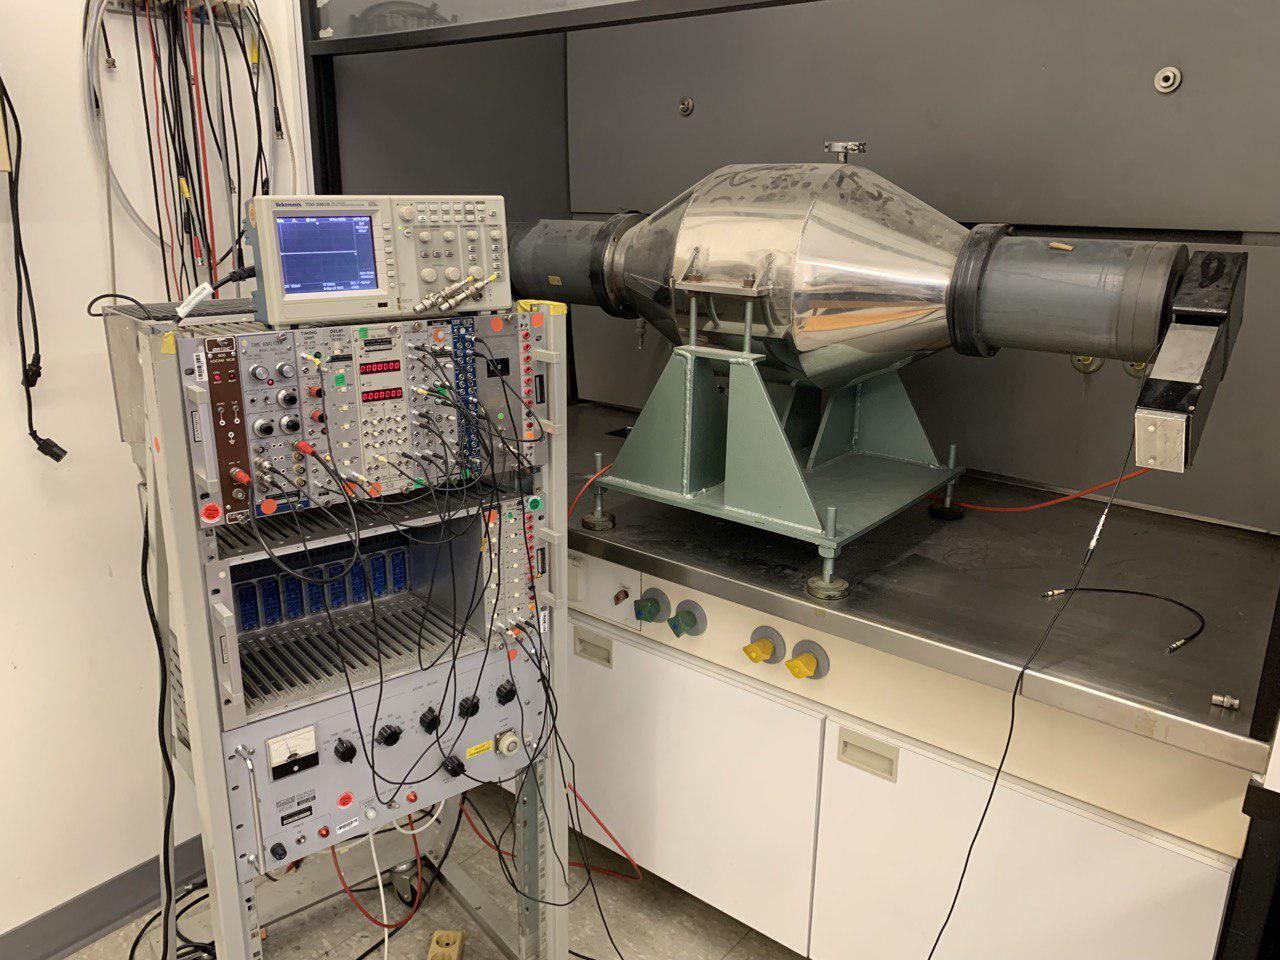
\includegraphics[width=0.7\linewidth]{figures/Aufbau_Foto.jpg}
    \caption{Foto des Versuchsaufbaus.}
    \label{fig:Aufbau_Foto}
\end{figure}
\FloatBarrier
\begin{figure}
    \centering
    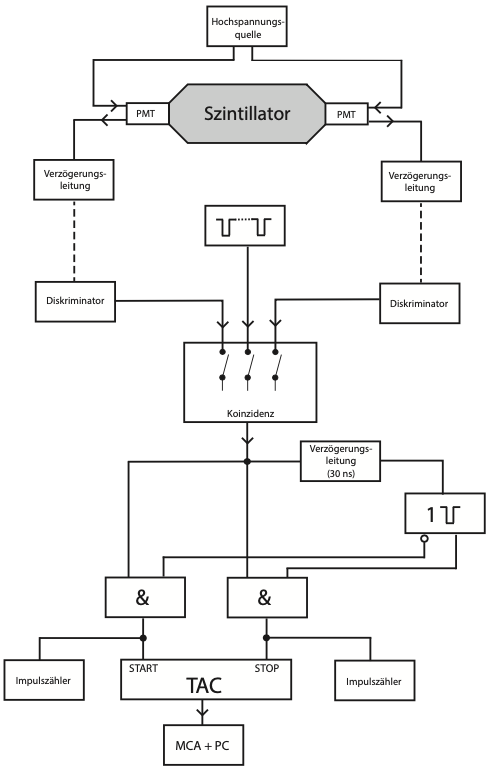
\includegraphics[width=0.7\linewidth]{figures/Aufbau.png}
    \caption{Blockschaltbild der Versuchsvorrichtung. \cite{V01}}
    \label{fig:Aufbau}
\end{figure}
\FloatBarrier


\subsection{Kalibrierung und Verkabelung}
Zunächst werden die am Szintillationstank angebrachten Photomultiplier an ein Oszilloskop angeschlossen, um sicherzustellen, dass sie funktionieren.
Anschließend werden die Photomultiplier über die Verzögerungsleitungen mit den Diskriminatoren verkabelt. Es wird noch keine Verzögerung eingestellt. Das Ergebnis wird ebenfalls am Oszilloskop sichtbar gemacht. An den Diskriminatoren wird die Pulsweite mithilfe der am Oszilloskop abgebildeten Pulse auf jeweils $\Delta t = \SI{10}{\nano\second}$ gestellt.
Als nächstes werden die Ausgänge der Diskriminatoren an einen Impulszähler angeschlossen. Die Schwelle der Diskriminatoren wird so angepasst, dass an beiden Ausgängen ca. $\num{30}$ Pulse pro Sekunde gemessen werden.
Im nächsten Schritt wird die Koinzidenz in die Schaltung integriert und der Ausgang an den Impulszähler angeschlossen. Die Verzögerungen werden systematisch nacheinander variiert. Dabei wird für jede Verzögerung die Impulsrate aufgenommen. Es ist ein deutliches Maximum, bzw. ein Plateau in der Verteilung, der Impulsrate zu sehen. Die Verzögerung wird auf diesen Wert eingestellt.
Die restliche Schaltung wird verkabelt. 
Am Monoflop wird eine Suchzeit $T_\text{s}$ eingestellt, die am auch TAC entsprechend eingestellt wird.

Der Teil vor der Koinzidenzschaltung wird abgeklemmt. Stattdessen wird ein Doppelimpulsgenerator an die Koinzidenz angeschlossen.
Die Pulsabstände werden zwischen $\SI{0.3}{\micro\second}$ und $\SI{9.9}{\micro\second}$ variiert und die entsprechende Kanalnummer des Vielkanalanalysators aufgenommen.

\subsection{Messung}
An die Koinzidenzschaltung werden erneut die zuvor abgeklemmten Photomultiplier angeschlossen. Die Aufzeichung des Vielkanalanalysators wird gleichzeitig mit dem Impulszähler gestartet und etwa $\num{20}$ bis $\SI{30}{\hour}$ laufen gelassen. %wie lange genau? Weiß man das? 

\newpage
\section{Auswertung}
Im folgenden Kapitel werden die gesammelten Messdaten sowie die Justierung der Koinzidenz und 
die Kalibrierung des Multichannel Analyzers ausgewertet.


\subsection{Justierung der Koinzidenz}
Vor Beginn der eigentlichen Messung muss die Koinzidenzschaltung justiert werden.
Treffen zwei Impulse auf die Koinzidenzschaltung werden beide Signale
zu einer logischen 1 zusammengeführt und weitergeleitet. 
%Die Bedingung, welche dafür erfüllt sein muss ist, dass die Impulse 
%nahezu gleichzeitig an der Koinzidenzschaltung eintreffen.
%Um dafür zu sorgen, dass die Signale welche zuvor aus den Diskriminatoren stammen genau dies tun,
%werden mit Hilfe von Verzögerungsleitungen unterschiedliche Signallaufzeiten erzeugt. 
%Da in der Wirklichkeit keine perfekte Gleichzeitigkeit realisiert werden kann, wird als 
%Aufweichung dieser Bedingung ein Zeitintervall $\Delta t$ definiert, indem wenn dort zwei Signale eintreffen sie
%als gleichzeitig eintreffend angesehen werden.
Der Zweck der Koinzidenzschaltung besteht darin, dass mit ihr überprüft werden kann, ob die Anzahl der 
detektierten Signale, eintreffende Myonen, mit dem theoretischen Erwartungswerts übereinstimmt.

Für die Justierung wird jeweils eine der Verzögerungleitungen in ihren Wert 
verändert und die resultierende Zählrate pro 10 Sekunden wird aufgenommen.
Anhand der messbaren Zählrate lässt sich erkennen, wann die optimale Verzögerung eingestellt ist.
Dies ist dann der Fall, wenn die Zählrate über verschieden eingestellte Verzögerungsdauern 
annähernd Konstant bleibt, sprich ein Plateau zeigt.
Das Plateau sollte in der Theorie $\SI{20}{\nano\second}$ breit sein, da die Diskriminatorpulse
jeweils eine eingestellt Länge von $\SI{10}{\nano\second}$ besitzen. 
Somit ist der maximale Überlagerungszeitraum genau die doppelte Pulslänge. 

Werden die unterschiedlichen Verzögerungsdauern in Abhängigkeit der Zählrate 
vgl. \autoref{tab:Koinzidenz} aufgetragen, lässt sich die Halbwertsbreite (FWHM) der Verteilung berechnen.
Der resultierende Graph ist in \autoref{fig:koinzidenz} zu sehen.
Die Fehler der Messwerte sind nach $\sqrt{N}$ gebildet worden, also dem Poisson-Fehler für Zählexperimente.
Zur Berechnung der Halbwertsbreite wird an beiden Flanken in \autoref{fig:koinzidenz}
eine lineare Regression durchgeführt.

Die Halbwertsbreite ergibt sich zu
\begin{equation}
    \text{FWHM} = |-22| + |16| = \SI{38}{\nano\second} \, ,
\end{equation}
bei einer Ereignisrate von $\SI{114,40 \pm 1,50}{\frac{1}{10 \second}}$ .
\begin{figure}
    \centering
    \includegraphics[width=0.7\linewidth]{build_new/plateau.pdf}
    \caption{Gemessene Signalrate in Abhängigkeit der Verzögerungen.}
    \label{fig:koinzidenz}
\end{figure}
\FloatBarrier
%\input{build/tabKoinzidenz.tex} %OLD
\input{build_new/tabKoinzidenz_new.tex} %FELIX
\input{build_new/tabKalibration_new.tex} %FELIX
\FloatBarrier

\subsection{Kalibrierung des Multichannel Analyzers}
Um den MCA zu kalibrieren, werden %TODO in der durchführung einführen -> erledigt
mit Hilfe eines Doppelimpulsgenerators Impulse mit unterschiedlichen Impulsabständen auf den MCA geschickt und von diesem verarbeitet.
Dadurch kann am Computer jeweils pro Impuls der jeweilige Kanal abgelesen werden.
Mit Hilfe dieser Wertepaare vgl.\autoref{tab:Kalibration} kann im Folgenden eine lineare Regression der Werte erfolgen und somit 
kann jedem Kanal des MCA eine Zeit zugeordnet werden. 
Im \autoref{fig:kalibration} ist die lineare Regression der Messwert zu sehen.
\begin{figure}
    \centering
    \includegraphics[width=0.7\linewidth]{build_new/kal.pdf}
    \caption{Graphische Darstellung der linearen Regression.}
    \label{fig:kalibration}
\end{figure}
\FloatBarrier
Die Regression liefert die Werte
\begin{equation}\label{eq:Regression}    
    \begin{split}
        m &= \num{0,04515(8)}\frac{\si{\micro\second}}{\text{Kanal}} \\
        b &= \SI{-0,041(10)}{\micro\second} \, .
    \end{split}
\end{equation}
\subsection{Bestimmung des Untergrunds}
Um den Untergrund zu bestimmen, muss zunächst berechnet 
werden wie viele Myonen im Mittel den Tank durchquert 
haben. 
\begin{equation}
  \overline{N} = \frac{N_{\symup{start}}}{T_{\symup{gesamt}}} \, .
\end{equation}
$N_\text{Start}$ steht hierbei für die Myonen, welche einen
Startimpuls ausgelöst haben.
Während der Suchzeit $T_\text{s}$ tun dies im Mittel
$n= \overline{N} \cdot T_\text{s}$ Myonen.
Anschließend wird mit Hilfe der Poissonverteilung die Anzahl
der Fehlmessungen bestimmt, also genau der Fall betrachtet falls zwei 
Myonen unmittelbar hintereinander den Detektor passieren 
sollten.
Anzumerken ist, dass die Startimpulse ebenfalls fehlerbehaftet ist. 
Der Fehler der Startimpulse bestimmt sich ebenfalls als Poisson-Fehler.
$N_{\symup{start}} = 3061879 \pm 1749$, $T_\text{s} = \SI{20}{\micro\second}$ und $T_{\symup{gesamt}}
= \SI{147182}{\second}$.
\begin{equation}
    N_{\symup{fehl}} = \overline{N} \cdot T_\text{s} \cdot \symup e^{- \overline{N} \cdot T_\text{s}}
    \cdot N_{\symup{start}} = \num{1273.4(15)} \, .
\end{equation}
Da sich dieser Fehler auf alle Kanäle gleichermaßen 
auswirkt, ergibt sich eine Untergrundrate von 
\begin{equation}
    U = \frac{N_{\symup{fehl}}}{\text{Anzahl Kanäle}} = \num{2.8298(32)} \, 
\end{equation}
mit 450 befüllten Kanälen.

\subsection{Bestimmung der Lebensdauer}
Im letzten Abschnitt wird die Lebensdauer der Myonen bestimmt.
Durch die Kalibration des MCA lässt sich jedem Kanal eine Zeit zuordnen, sodass 
mit den unterschiedlichen Ereignisraten der Graph in \autoref{fig:fit} entsteht.
Die Exponentialfunktion mit der die Messdaten gefittet werden, lautet
\begin{equation}
    N(t) = N_0 \cdot \symup e^{-\lambda \, t} + U \, .
    \label{fit}
\end{equation}
Hierbei steht $U$ für die zuvor berechnete Untergrundrate.
Die Parameter des Fits sind
\begin{align}
    N_0 &= \num{241.8(13)} \ \text{pro Kanal} \\
    \lambda &= \SI{0.456(5)}{\per\micro\second} \label{dauer}\, .% \\
    %U_{\symup{fit}} &= \num{1.8(13)} \ \text{pro Kanal} \label{Untergrund} \, .
\end{align}
Der inverse Abklingkoeffizient liefert schließlich die Lebensdauer des Myons.
Diese ist 
\begin{equation}
    \tau = \SI{2.20(2)}{\micro\second} \, .
\end{equation}
\begin{figure}
    \centering
    \includegraphics[width=0.7\linewidth]{build_new/fit.pdf}
    \caption{Gefittete Ereignisrate in Abhängigkeit der Zeit.}
    \label{fig:fit}
\end{figure}


\section{Diskussion}
%TODO kann ich nicht die erwartete anzahl der eriegnisse mit den gemessenen vergelcihen
%was genau muss ich mit der fwhm machen und was sagt diese aus?
%
Die Messung der Halbwertsbreite der Koinzidenzschaltung liefert einen Wert von $\text{FHWM} = \SI{38}{\nano\second}$.
Damit weicht die gemessene Halbwertsbreite vom erwarteten Wert $\text{FHWM} = \SI{20}{\nano\second}$ um 47\,\% ab.
Der wahrscheinlichste Grund für diese Abweichung ist, dass die Pulslänge welche der Diskriminator liefert
über $\SI{10}{\nano\second}$ liegt.
Somit ist der Überlagerungszeitraum der beiden Pulse länger.

Die im Experiment ermittelte Lebensdauer des Myons $\tau = \SI{2.20(2)}{\micro\second}$ 
besitzt eine Abweichung zum
Literaturwert $\tau = \SI{2.197}{\micro\second}$ \cite{lebensdauer} von 1,04\,\%.
Damit kann der ermittelte Wert als plausibel angenommen werden.
Die geringe Abweichung ist wahrscheinlich auf die hohe Ereignisrate zurückzuführen,
da die statistischen Abweichungen mit Erhöhung der Messungen sinken.
Die durchgeführte Ausgleichsrechnung kommt dadurch dem tatsächlichen Verlauf der Zählrate näher.
Andere kleinere Fehlerquellen sind beispielsweise die Justierung der Suchzeit am Monoflop per Hand oder
das Einstellen des Diskriminators mit Hilfe eines Schraubendrehers. 

Die Suchzeit des Monoflop beträgt im Experiment $T_\text{s}= \SI{20}{\micro\second}$.
Würde die Suchzeit am Monoflop beispielsweise auf $\SI{5}{\micro\second}$ verkürzt werden, 
wäre zwar immer noch eine Verteilung
der Myonen messbar, aber der Graph in \autoref{fig:fit} würde bereits nach $\SI{5}{\micro\second}$ enden.
Um also effektiv eine vergleichbare Messgenauigkeit der Lebensdauer zu kommen, müsste deutlich
länger gemessen werden.
Wird die Suchzeit hingegen vergrößert besteht die Gefahr, dass zwei eigentliche Startimpulse 
fälschlicherweise als Start und Stop Signal gewertet werden. 
Dadurch würde die Lebensdauer verfälscht.

Wird die einstellbare Schwelle am Diskriminator erhöht, so müsste ebenfalls länger gemessen werden um 
auf eine vergleichbar genaue Lebensdauer zu kommen.
Nur solche Myonen, welche eine sehr starken Lichtblitz auslösen können den Diskriminator passieren.
Wenn hingegen die Schelle zu klein angesetzt wird, wird zu viel Rauschen des Szintillator weitergeleitet.
Damit würde die Koinzidenzschaltung permanent ausgelöst werden und auch der Monoflop würde 
permanent Start und Stop Signale registrieren. 
Damit wäre keine Lebensdauerbestimmung mehr möglich.


\nocite{*}
\printbibliography{}
\end{document}
%\begin{figure}
%    \centering
%    \includegraphics[width=0.7\linewidth]{./figures/xxx.xxx}
%    \caption{xxx}
%    \label{fig:xxx}
%\end{figure}
%
%\begin{equation}\label{eq:xxx}    
%    \begin{split}
%        \lambda &= \SI{855}{\angstrom}\\
%        \delta_\text{ps} &= 0,6\cdot 10^{-6}\\
%        \delta_\text{si}&= 6,8\cdot 10^{-6} \\
%        n_\text{luft} &= 1 \\
%        n_\text{ps} &= 1 - \delta_\text{ps} \\
%        n_\text{si} &= 1 - \delta_\text{ps} 
%    \end{split}
%\end{equation} 